\documentclass[11pt,a4paper]{article}

% ── Paquetes ─────────────────────────────────────────────────────────────
\usepackage[utf8]{inputenc}
\usepackage[spanish]{babel}
\usepackage[T1]{fontenc}
\usepackage[margin=2.5cm]{geometry}
\usepackage{graphicx} % Required for inserting images
\usepackage{booktabs}
\usepackage{caption}
\usepackage{float}
\usepackage{amsmath}
\usepackage{xcolor}
\definecolor{NavyBlue}{HTML}{1A3A6B}
\usepackage[colorlinks=true, linkcolor=NavyBlue, citecolor=NavyBlue, urlcolor=NavyBlue]{hyperref}

\graphicspath{{eda_ml_figs/}{assets/}{assets/authors/}}

% \title/\author solo alimentan los metadatos del PDF (via hyperref); la
% portada visual se arma a mano abajo con \begin{titlepage}, así que no se
% llama a \maketitle (evitaría una segunda portada duplicada).
\title{EDA — Mercado Laboral Colombiano}
\author{Santiago Hurtado, Juan Marín, Andrés Parejo}
\date{Agosto 2026}

\begin{document}

\begin{titlepage}
    \centering
    
\includegraphics[height=2.2cm]{un_logo.png}\hspace{1.5cm}
    
\includegraphics[height=2.2cm]{banrep_logo.png}

    \vspace{3cm}
    {\Huge\bfseries EDA — Mercado Laboral Colombiano\par}
    \vspace{0.5cm}
    {\Large Análisis exploratorio de datos como preparación para un modelo de Machine Learning\par}

    \vspace{2cm}
    {\large Santiago Hurtado \quad Juan Marín \quad Andrés Parejo\par}
    \vspace{0.3cm}
    {\large Universidad del Norte — Ciencia de Datos\par}

    \vspace{2cm}
    {\large Agosto de 2026\par}

    \vfill
    {\small Fuente de datos: DANE / Banco de la República\par}
\end{titlepage}

\begin{abstract}
Este documento presenta el análisis exploratorio de datos (EDA) de las series históricas del mercado laboral colombiano publicadas por el DANE y distribuidas por el Banco de la República, para el período enero de 2001 a diciembre de 2025 (300 observaciones mensuales). Se examinan seis series —tasa global de participación, tasa de desempleo y tasa de ocupación, cada una a nivel de 13 áreas metropolitanas y nacional— con el objetivo de caracterizar su distribución, identificar valores atípicos, cuantificar la multicolinealidad entre variables y evaluar la estacionariedad y estacionalidad de la tasa de desempleo nacional, variable objetivo de un futuro modelo predictivo.
\end{abstract}

\tableofcontents
\newpage

% ══════════════════════════════════════════════════════════════════════════
\section{Introducción}
% ══════════════════════════════════════════════════════════════════════════

Este análisis exploratorio parte de las series históricas del mercado laboral colombiano publicadas por el Departamento Administrativo Nacional de Estadística (DANE) a partir de la Gran Encuesta Integrada de Hogares (GEIH), y distribuidas por el Banco de la República dentro de su portal de series estadísticas históricas.

\subsection{Contexto del dataset}

\begin{table}[H]
    \centering
    \caption{Metadatos del dataset}
    \begin{tabular}{ll}
        \toprule
        \textbf{Atributo} & \textbf{Valor} \\
        \midrule
        Periodicidad & Mensual \\
        Unidad de medida & Porcentaje (\%) \\
        Fuente & DANE / Banco de la República \\
        Disponible desde & 2001-01-31 \\
        Disponible hasta & 2025-12-31 \\
        Observaciones & 300 \\
        Descargado & 27/02/2026 \\
        \bottomrule
    \end{tabular}
\end{table}

El conjunto de datos contiene 300 observaciones mensuales (25 años completos) y 6 series correspondientes a tres indicadores del mercado laboral, cada uno medido a nivel de las 13 principales áreas metropolitanas y a nivel nacional:

\begin{itemize}
    \item \textbf{Tasa Global de Participación (TGP) — 13 áreas / Nacional.} Relación porcentual entre la población que integra la fuerza de trabajo y la población en edad de trabajar (PET). Refleja la presión de la PET sobre el mercado laboral.
    \item \textbf{Tasa de Desempleo (TD) — 13 áreas / Nacional.} Relación porcentual entre el número de personas desocupadas y el número de personas que integran la fuerza de trabajo (FT). Es la variable objetivo de este estudio.
    \item \textbf{Tasa de Ocupación (TO) — 13 áreas / Nacional.} Relación porcentual entre la población ocupada y la población en edad de trabajar (PET).
\end{itemize}

\subsection{Interpretación preliminar}

El mercado laboral colombiano es un indicador central del desempeño económico del país: refleja tanto la capacidad de la economía para generar empleo como la presión que ejerce la población en edad de trabajar sobre ese mercado. Las tres tasas que componen este dataset —participación, desempleo y ocupación— están matemáticamente relacionadas (la PET se reparte entre fuerza de trabajo e inactivos, y la fuerza de trabajo entre ocupados y desocupados), por lo que es esperable observar una fuerte correlación negativa entre desempleo y ocupación, y una relación más débil con la participación.

Los 300 meses del dataset muestran una tasa de desempleo nacional que se movió entre 7.02\% (noviembre de 2025) y 21.97\% (mayo de 2020), con una media de 11.61\%. El episodio más disruptivo del periodo es, sin sorpresa, la pandemia de COVID-19: el máximo histórico se registra en plena crisis sanitaria, más de 8 puntos por encima de la media. Fuera de ese choque, la serie muestra una tendencia estructural a la baja entre 2001 y 2015, seguida de una relativa estabilización.

Para efectos del modelo predictivo que se construirá a futuro, este comportamiento sugiere dos cosas: (1) la serie no es estacionaria y tiene estacionalidad anual, por lo que requerirá diferenciación antes de modelarse, y (2) el periodo COVID debe tratarse explícitamente (por ejemplo, como variable \textit{dummy}) en lugar de eliminarse, ya que es información real y no un error de medición.

\newpage
% ══════════════════════════════════════════════════════════════════════════
\section{Análisis Exploratorio de Datos (EDA)}
% ══════════════════════════════════════════════════════════════════════════

\subsection{Inspección inicial}

El dataset no presenta valores faltantes, fechas duplicadas, ni saltos en la periodicidad mensual; el orden cronológico es correcto. La Tabla~\ref{tab:desc} resume los estadísticos descriptivos de las seis variables.

\begin{table}[H]
    \centering
    \caption{Estadísticos descriptivos}
    \label{tab:desc}
    \resizebox{\textwidth}{!}{%
    \begin{tabular}{lrrrrrrrr}
        \toprule
        \textbf{Variable} & \textbf{Media} & \textbf{DS} & \textbf{Min} & \textbf{Q1} & \textbf{Mediana} & \textbf{Q3} & \textbf{Max} & \textbf{IQR} \\
        \midrule
        Desempleo (nacional)      & 11.612 & 2.449 & 7.020  & 9.735  & 11.193 & 12.909 & 21.972 & 3.174 \\
        Participación (área)      & 67.759 & 2.224 & 55.088 & 66.565 & 67.954 & 69.469 & 72.148 & 2.904 \\
        Participación (nacional)  & 65.740 & 2.346 & 53.446 & 64.087 & 66.139 & 67.482 & 70.618 & 3.395 \\
        Desempleo (área)          & 12.627 & 3.147 & 7.270  & 10.450 & 11.730 & 14.021 & 25.789 & 3.572 \\
        Ocupación (área)          & 59.218 & 3.097 & 41.658 & 57.706 & 59.588 & 61.128 & 64.610 & 3.422 \\
        Ocupación (nacional)      & 58.120 & 2.855 & 42.497 & 56.841 & 58.315 & 59.960 & 64.008 & 3.119 \\
        \bottomrule
    \end{tabular}%
    }
\end{table}

\subsection{Análisis univariado — variable objetivo}

La distribución de la tasa de desempleo nacional presenta sesgo positivo (\textit{skewness} = 1.09, curtosis = 1.65): la mayoría de los meses se concentra entre 9\% y 13\%, con una cola larga hacia valores altos causada por los picos de 2020. La media (11.61\%) queda por encima de la mediana (11.19\%), comportamiento típico cuando existen eventos extremos ocasionales.

\begin{figure}[H]
    \centering
    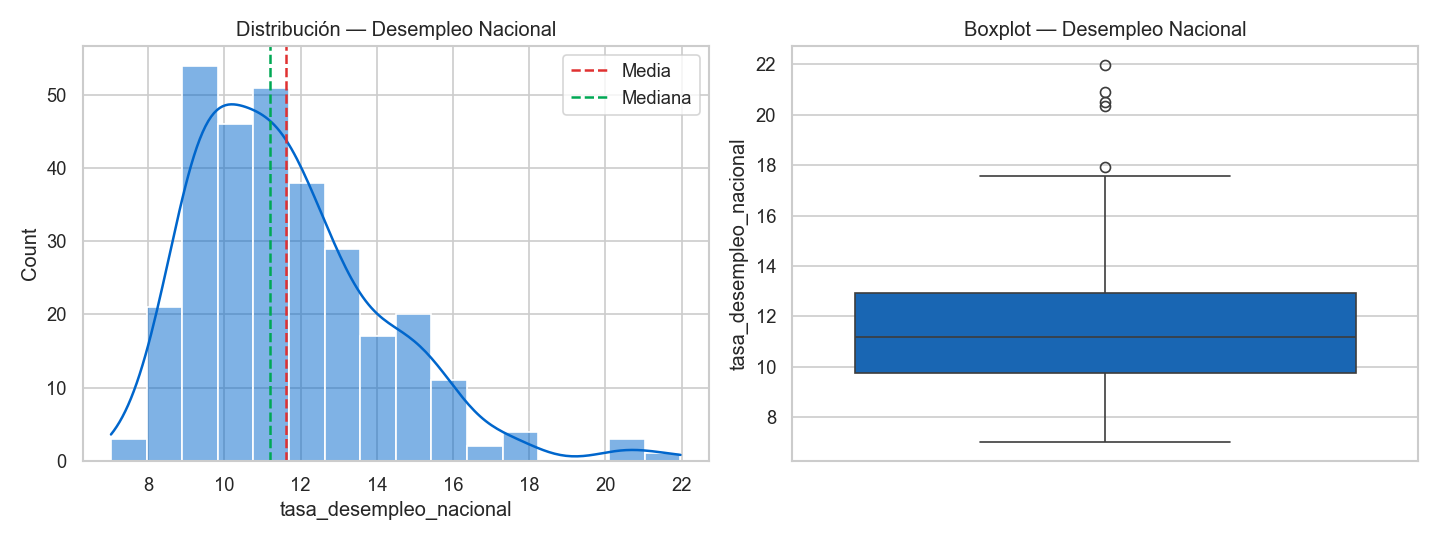
\includegraphics[width=0.85\textwidth]{01_univariado_target.png}
    \caption{Histograma y boxplot de la tasa de desempleo nacional}
\end{figure}

Aplicando la regla de 1.5×IQR se identifican 5 observaciones atípicas (Tabla~\ref{tab:outliers}), cuatro de ellas asociadas al choque del COVID-19. Se conservan en el análisis por representar información real del mercado laboral y no errores de medición.

\begin{table}[H]
    \centering
    \caption{Outliers en la tasa de desempleo nacional}
    \label{tab:outliers}
    \begin{tabular}{lr}
        \toprule
        \textbf{Fecha} & \textbf{Tasa de desempleo nacional} \\
        \midrule
        2002-01-31 & 17.91\% \\
        2020-04-30 & 20.49\% \\
        2020-05-31 & 21.97\% \\
        2020-06-30 & 20.36\% \\
        2020-07-31 & 20.91\% \\
        \bottomrule
    \end{tabular}
\end{table}

\begin{figure}[H]
    \centering
    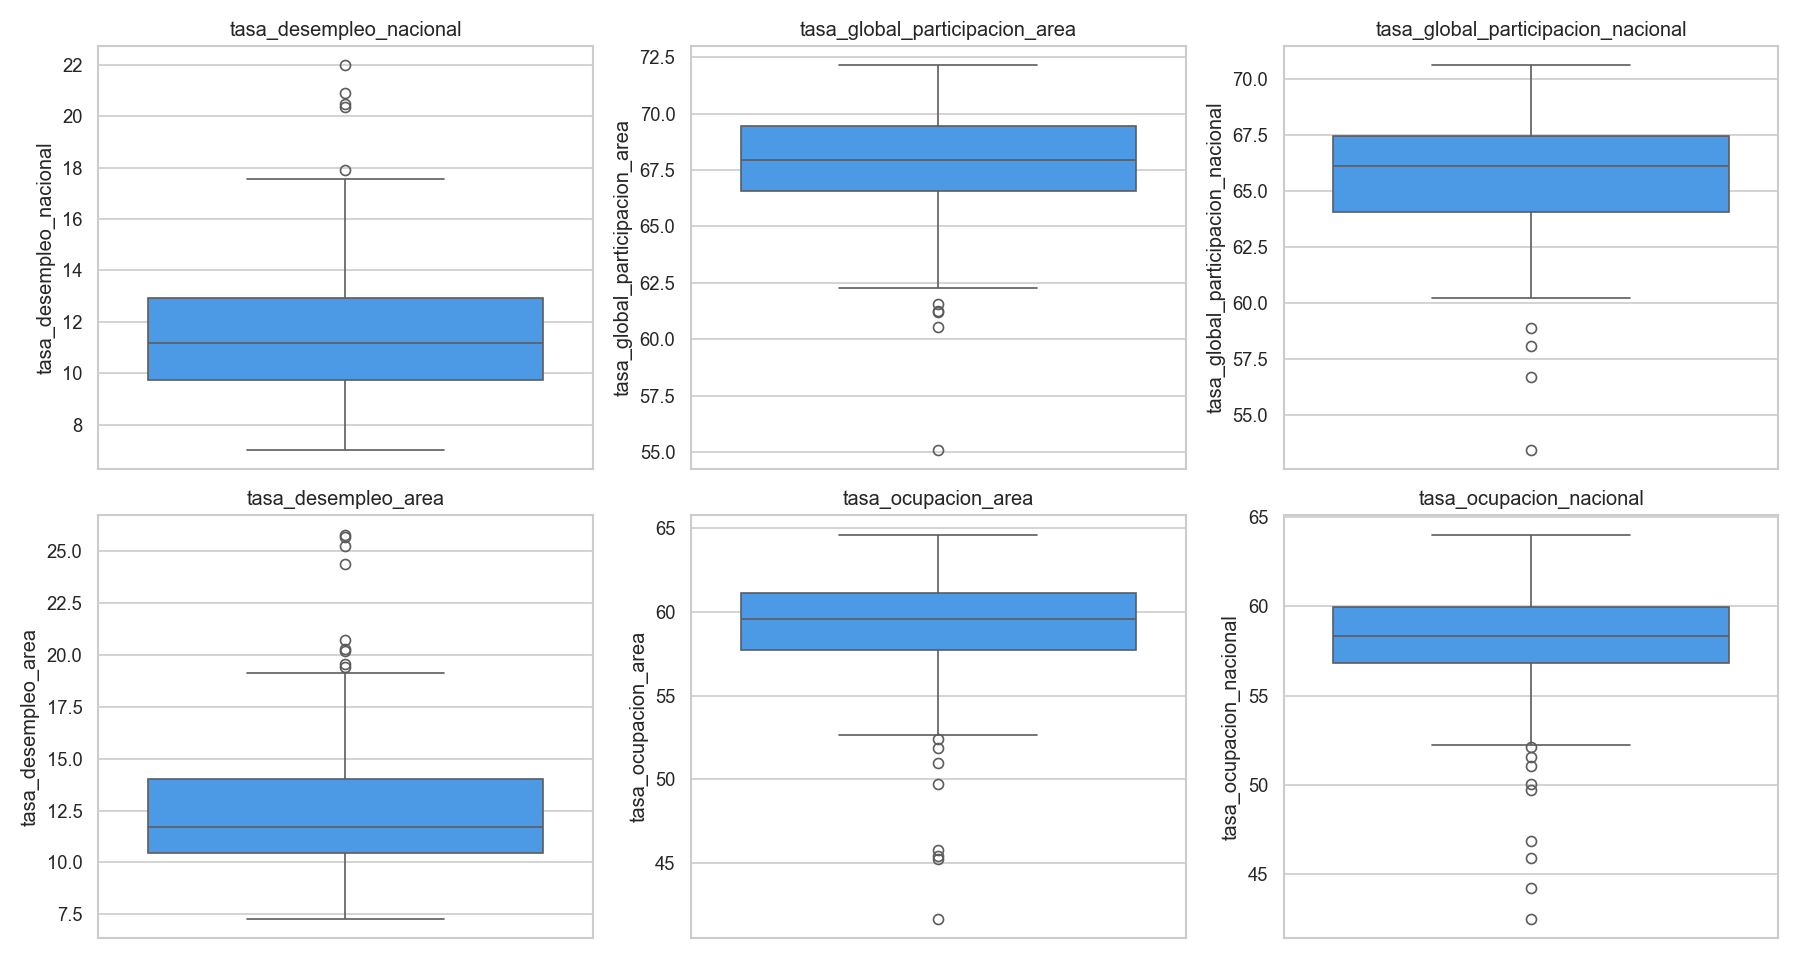
\includegraphics[width=\textwidth]{02_boxplots_todas_variables.png}
    \caption{Distribución por indicador — las tasas de ocupación y participación (42–72\%) tienen escalas más altas que las de desempleo (7–26\%), aunque todas se miden en porcentaje.}
\end{figure}

\subsection{Bivariado y multicolinealidad}

La Tabla~\ref{tab:corr} y la Figura~\ref{fig:corr} muestran que las correlaciones más fuertes se dan entre los pares área/nacional del mismo indicador (\textgreater 0.94), lo que sugiere redundancia informativa. El desempleo nacional correlaciona negativamente con la ocupación (\(-0.82\) con el área y \(-0.73\) con la nacional) y débilmente con la participación (\(-0.27\) con el área, \(-0.24\) con la nacional).

\begin{table}[H]
    \centering
    \caption{Matriz de correlación de Pearson}
    \label{tab:corr}
    \resizebox{\textwidth}{!}{%
    \begin{tabular}{lrrrrrr}
        \toprule
         & \textbf{TGP-A} & \textbf{TGP-N} & \textbf{TD-A} & \textbf{TD-N} & \textbf{TO-A} & \textbf{TO-N} \\
        \midrule
        TGP-A (Participación área)      & 1.000  & 0.949  & -0.206 & -0.269 & 0.749  & 0.822 \\
        TGP-N (Participación nacional)  & 0.949  & 1.000  & -0.159 & -0.239 & 0.684  & 0.841 \\
        TD-A (Desempleo área)           & -0.206 & -0.159 & 1.000  & 0.964  & -0.802 & -0.645 \\
        TD-N (Desempleo nacional)       & -0.269 & -0.239 & 0.964  & 1.000  & -0.817 & -0.725 \\
        TO-A (Ocupación área)           & 0.749  & 0.684  & -0.802 & -0.817 & 1.000  & 0.938 \\
        TO-N (Ocupación nacional)       & 0.822  & 0.841  & -0.645 & -0.725 & 0.938  & 1.000 \\
        \bottomrule
    \end{tabular}%
    }
\end{table}

\begin{figure}[H]
    \centering
    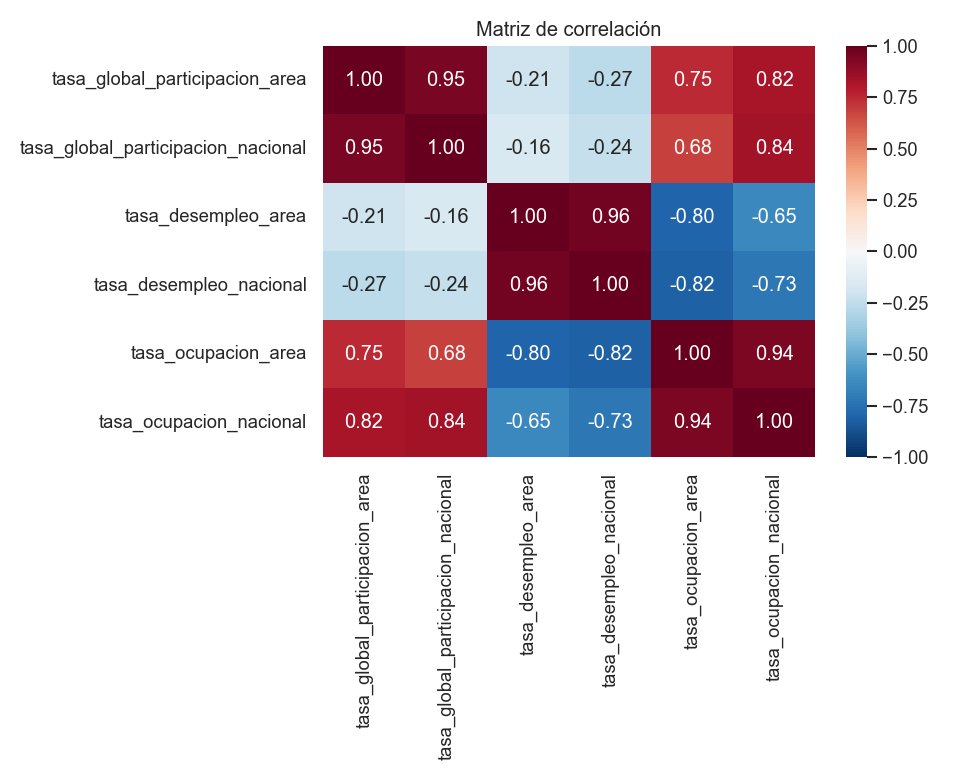
\includegraphics[width=0.7\textwidth]{03_correlacion.png}
    \caption{Matriz de correlación}
    \label{fig:corr}
\end{figure}

La Tabla~\ref{tab:vif} cuantifica esa redundancia mediante el factor de inflación de la varianza (VIF). Todas las variables predictoras superan ampliamente el umbral convencional de VIF = 10, confirmando multicolinealidad severa. Antes de ajustar un modelo lineal es necesario eliminar variables redundantes (por ejemplo, conservar solo la versión nacional o solo la de área de cada indicador) o aplicar una técnica de reducción de dimensionalidad.

\begin{table}[H]
    \centering
    \caption{Factor de Inflación de la Varianza (VIF)}
    \label{tab:vif}
    \begin{tabular}{lr}
        \toprule
        \textbf{Variable} & \textbf{VIF} \\
        \midrule
        Ocupación (área)          & 959.46 \\
        Participación (área)      & 402.04 \\
        Desempleo (área)          & 385.32 \\
        Ocupación (nacional)      & 52.16 \\
        Participación (nacional)  & 48.54 \\
        \bottomrule
    \end{tabular}
\end{table}

\begin{figure}[H]
    \centering
    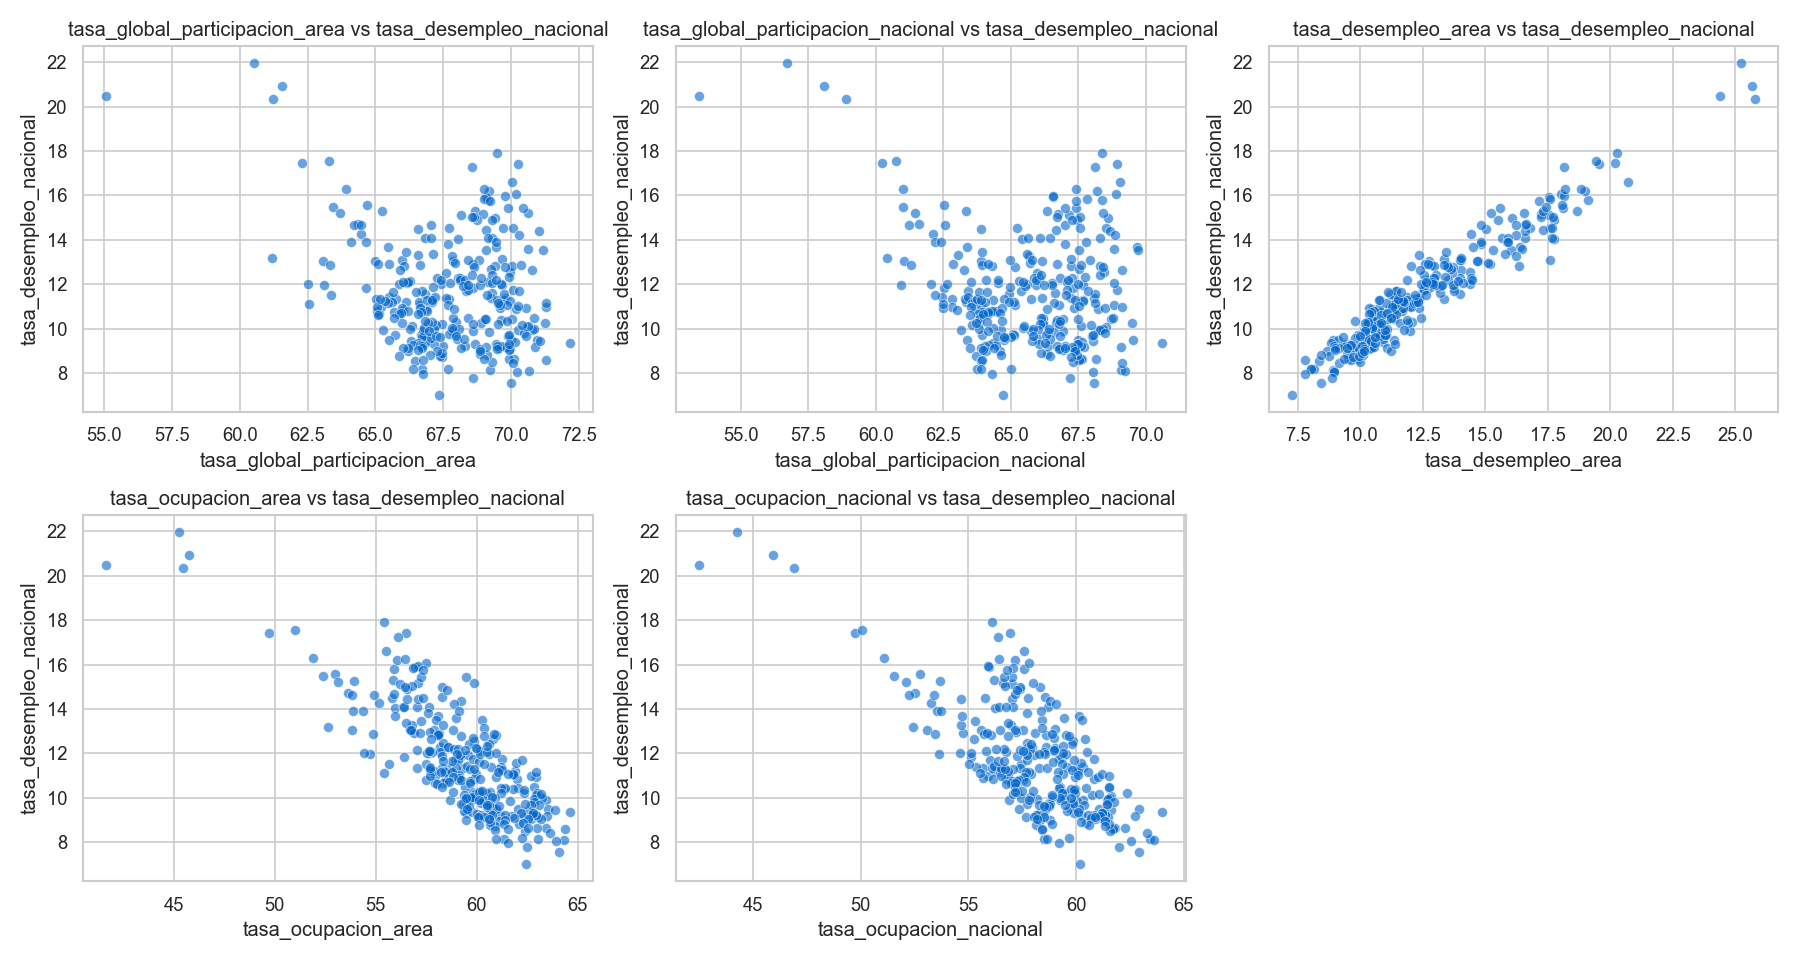
\includegraphics[width=\textwidth]{04_dispersion_target_vs_features.png}
    \caption{Dispersión de la tasa de desempleo nacional contra cada variable predictora. La relación con la ocupación nacional es la más clara y negativa; con las tasas de participación es más difusa, ya que entrar a la fuerza laboral no siempre implica desempleo.}
\end{figure}

\subsection{Evolución temporal}

Desempleo y ocupación nacional se mueven en direcciones opuestas durante casi todo el periodo. El quiebre más marcado ocurre en 2020: el desempleo se dispara mientras la ocupación cae abruptamente por las restricciones asociadas a la pandemia de COVID-19.

\begin{figure}[H]
    \centering
    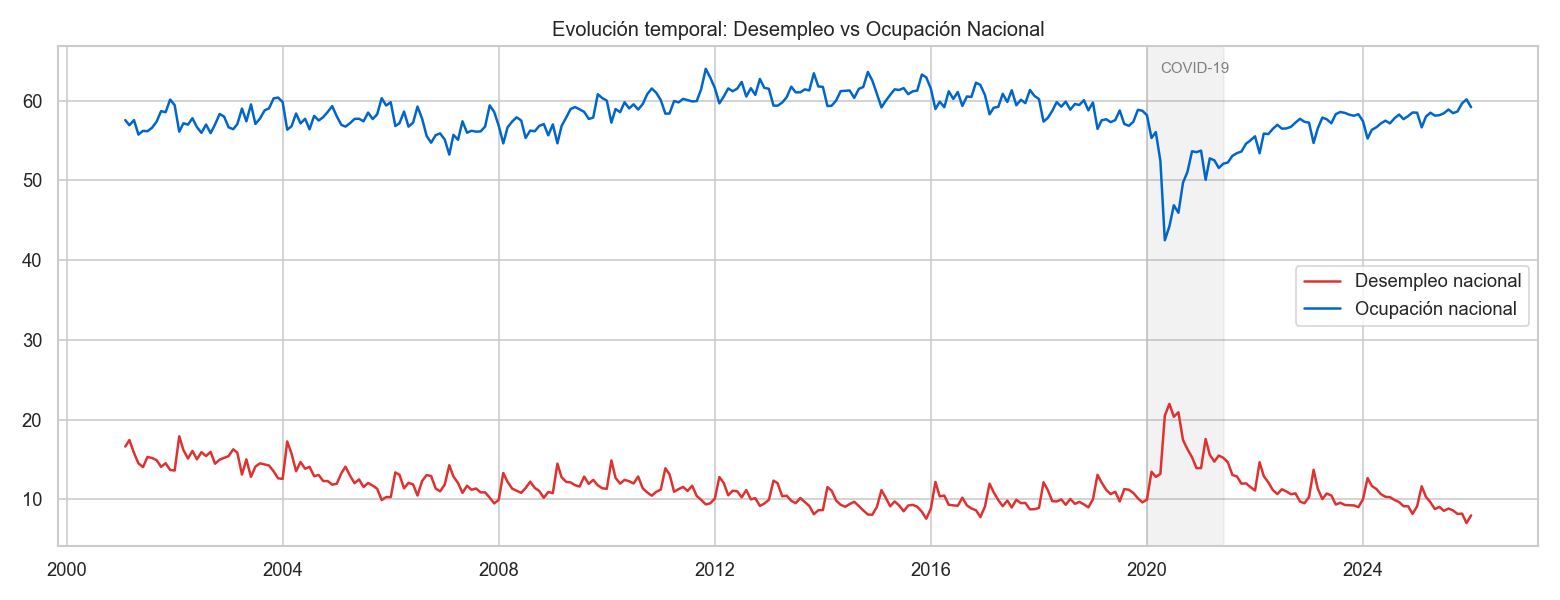
\includegraphics[width=\textwidth]{05_evolucion_temporal.png}
    \caption{Evolución temporal — Desempleo vs. Ocupación Nacional}
\end{figure}

\begin{figure}[H]
    \centering
    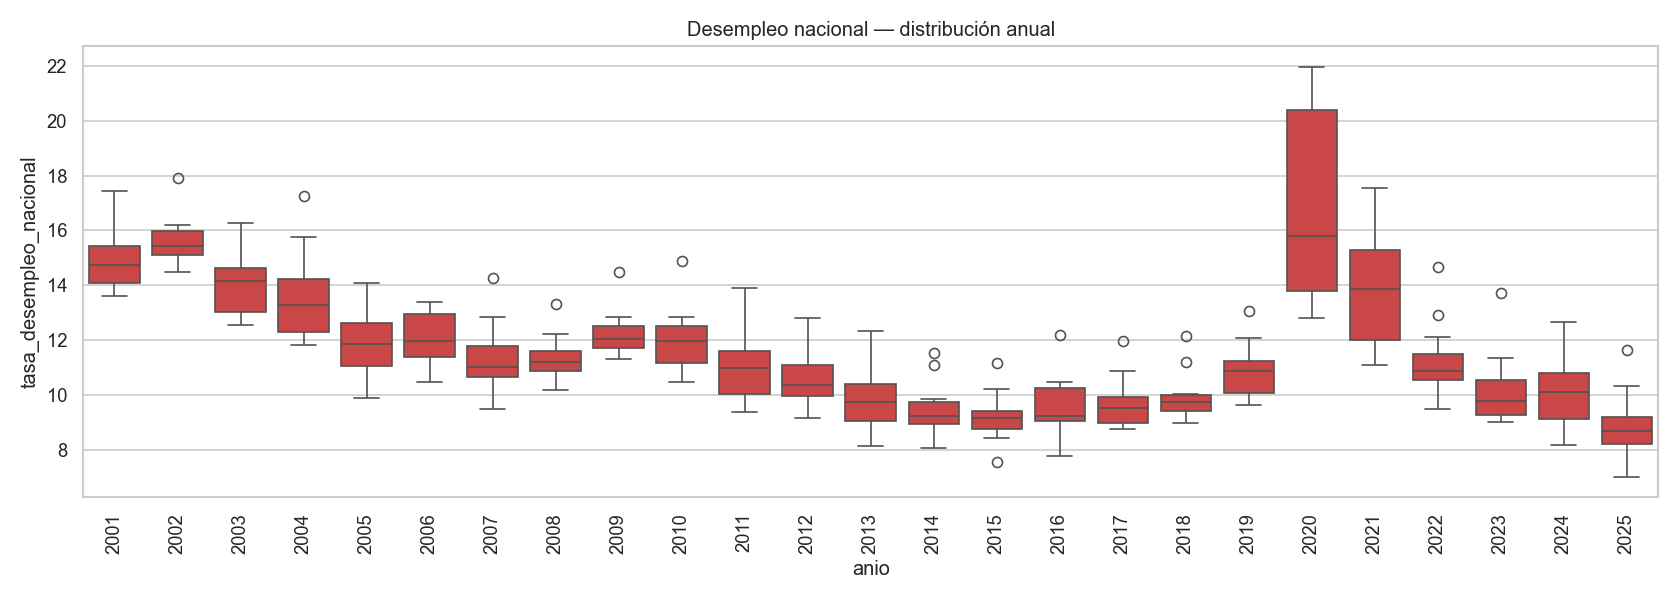
\includegraphics[width=0.85\textwidth]{06_boxplot_anual.png}
    \caption{Distribución anual de la tasa de desempleo nacional. La mediana desciende de forma sostenida entre 2001 y 2015, se estabiliza, y repunta bruscamente en 2020 antes de retomar la tendencia decreciente hasta 2025.}
\end{figure}

\subsection{Estacionariedad y estacionalidad}

Se aplicó la prueba de Dickey-Fuller Aumentada (ADF, \(H_0\): la serie tiene raíz unitaria / no es estacionaria) a las seis series, no solo a la variable objetivo, dado que todas son candidatas a variables predictoras del futuro modelo (Tabla~\ref{tab:adf}). Ninguna de las series es estacionaria en niveles, con la excepción marginal de la tasa de desempleo por área (\(p = 0.045\)).

\begin{table}[H]
    \centering
    \caption{Prueba ADF por variable}
    \label{tab:adf}
    \begin{tabular}{lrrrl}
        \toprule
        \textbf{Variable} & \textbf{Estadístico ADF} & \textbf{p-valor} & \textbf{N lags} & \textbf{Estacionaria} \\
        \midrule
        Desempleo (nacional)     & -2.7285 & 0.0692 & 12 & No \\
        Participación (área)     & -1.4731 & 0.5468 & 13 & No \\
        Participación (nacional) & -1.8352 & 0.3631 & 12 & No \\
        Desempleo (área)         & -2.8993 & 0.0454 & 12 & Sí \\
        Ocupación (área)         & -2.2570 & 0.1862 & 12 & No \\
        Ocupación (nacional)     & -2.2873 & 0.1761 & 12 & No \\
        \bottomrule
    \end{tabular}
\end{table}

La descomposición clásica multiplicativa (Figura~\ref{fig:decomp}) confirma la caída estructural del desempleo en 25 años (tendencia), un componente estacional que se repite cada 12 meses con amplitud estable, y residuos que se disparan en 2020 — señal de que ese periodo no lo explican ni la tendencia ni la estacionalidad.

\begin{figure}[H]
    \centering
    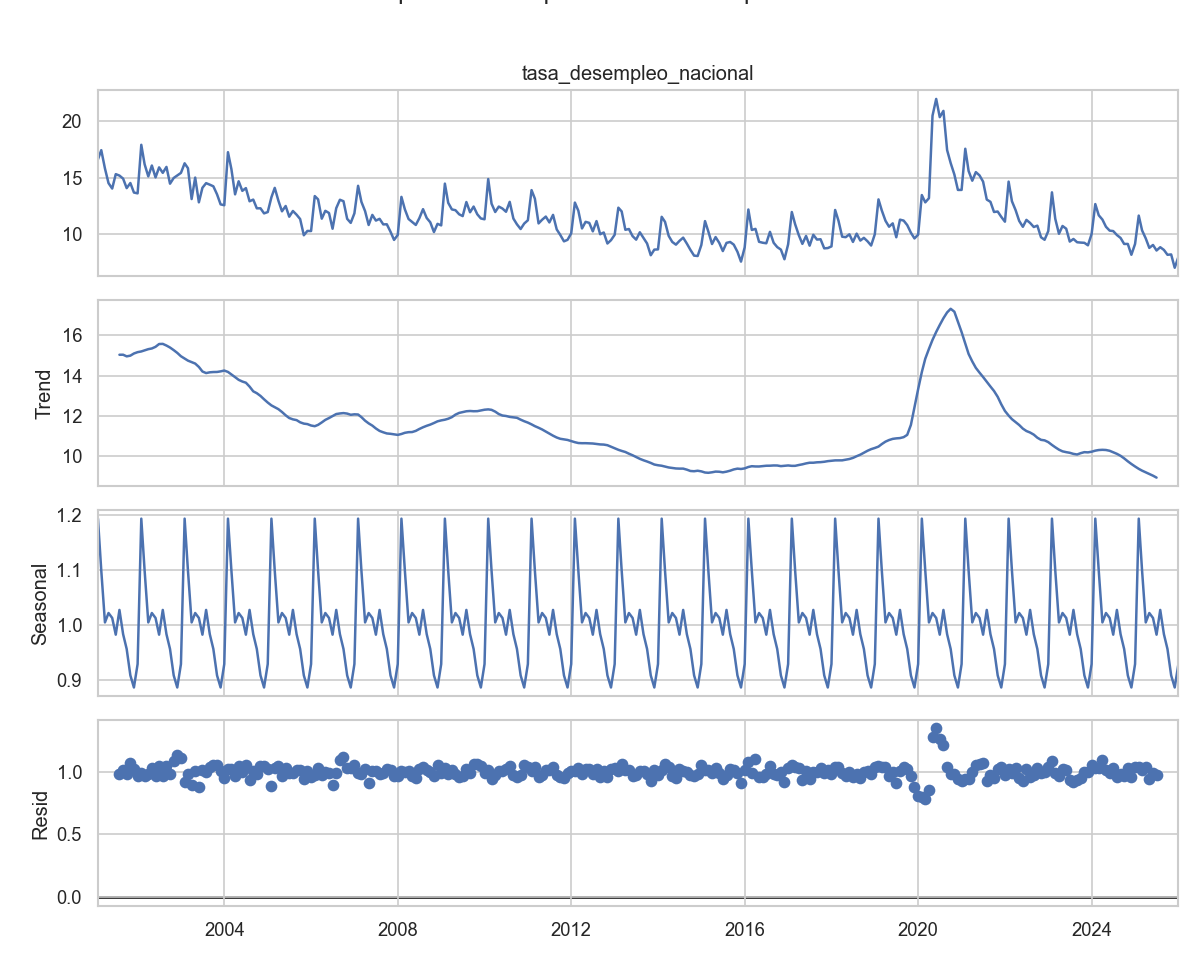
\includegraphics[width=0.85\textwidth]{07_descomposicion.png}
    \caption{Descomposición clásica multiplicativa — Desempleo Nacional}
    \label{fig:decomp}
\end{figure}

El correlograma (ACF) decae lentamente con picos en múltiplos de 12, evidencia adicional de no estacionariedad y estacionalidad anual. El PACF cae abruptamente tras los primeros rezagos, lo que sugiere un componente autorregresivo de orden bajo una vez diferenciada la serie — orientando el modelado hacia un esquema SARIMA\((p,1,q)(P,1,Q)_{12}\).

\begin{figure}[H]
    \centering
    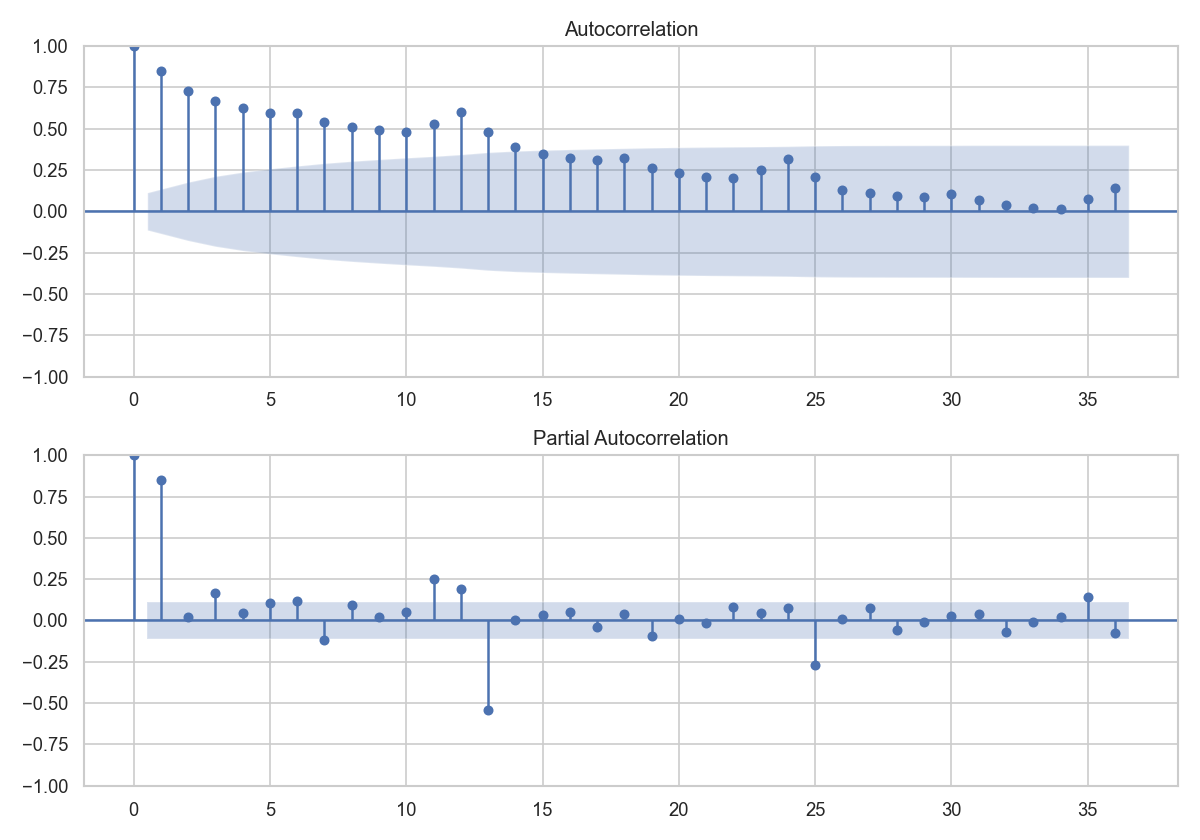
\includegraphics[width=0.85\textwidth]{08_acf_pacf.png}
    \caption{Serie, ACF y PACF — Desempleo Nacional}
\end{figure}

\subsection{Ingeniería de variables para el modelo}

A partir de los hallazgos anteriores se construyeron variables candidatas para el futuro modelo: rezagos de 1, 3, 6 y 12 meses de la tasa de desempleo nacional, medias y desviaciones móviles a 3, 6 y 12 meses, una variable de mes (estacionalidad) y una variable \textit{dummy} para el periodo COVID (enero de 2020 a junio de 2021).

La Tabla~\ref{tab:lags} muestra la correlación del target con sus propios rezagos: el de 1 mes es, por mucho, el predictor más fuerte del desempleo del mes siguiente; los rezagos estacionales (6 y 12 meses) también aportan información relevante.

\begin{table}[H]
    \centering
    \caption{Correlación del target con sus rezagos}
    \label{tab:lags}
    \begin{tabular}{lr}
        \toprule
        \textbf{Rezago} & \textbf{Correlación} \\
        \midrule
        lag 1  & 0.859 \\
        lag 3  & 0.694 \\
        lag 12 & 0.651 \\
        lag 6  & 0.627 \\
        \bottomrule
    \end{tabular}
\end{table}

\subsection{Split temporal train/test}

Para el futuro entrenamiento del modelo se definió un corte temporal (no aleatorio, como corresponde a una serie de tiempo) dejando los últimos 24 meses como conjunto de prueba:

\begin{itemize}
    \item \textbf{Train:} 276 observaciones (2001-01-31 a 2023-12-31).
    \item \textbf{Test:} 24 observaciones (2024-01-31 a 2025-12-31).
\end{itemize}

Este mismo corte —o una validación \textit{walk-forward}— debe usarse al entrenar el modelo; un split aleatorio filtraría información futura al entrenamiento.

\newpage
% ══════════════════════════════════════════════════════════════════════════
\section{Resumen de hallazgos}
% ══════════════════════════════════════════════════════════════════════════

\begin{itemize}
    \item Dataset completo, sin nulos ni duplicados — 300 observaciones mensuales, enero de 2001 a diciembre de 2025.
    \item 5 outliers en el target, 4 asociados al choque COVID-19 (2020) — se conservan por ser información real.
    \item Multicolinealidad severa confirmada por VIF entre variables de área y nacional — eliminar redundantes o aplicar PCA antes de modelos lineales.
    \item Ninguna de las 6 series es estacionaria en niveles — se requiere diferenciación; la estacionalidad anual es clara en la descomposición y el ACF.
    \item Los rezagos 1, 3 y 12 del target son los predictores más correlacionados — candidatos naturales de \textit{feature engineering}.
    \item Split temporal definido en 24 meses de test — usar este mismo corte o validación \textit{walk-forward} al entrenar, nunca un split aleatorio.
\end{itemize}

\newpage
% ══════════════════════════════════════════════════════════════════════════
\section{Autores}
% ══════════════════════════════════════════════════════════════════════════

\begin{minipage}[t]{0.31\textwidth}
    \centering
    
\includegraphics[width=0.9\textwidth]{parejo.png}\par
    \textbf{Andrés Parejo}\par
    \small Estudiante de ciencia de datos con enfoque en educación y programación.
\end{minipage}
\hfill
\begin{minipage}[t]{0.31\textwidth}
    \centering
    
\includegraphics[width=0.9\textwidth]{marin.png}\par
    \textbf{Juan Marín}\par
    \small Estudiante de ciencia de datos con enfoque en estadística y ML.
\end{minipage}
\hfill
\begin{minipage}[t]{0.31\textwidth}
    \centering
    
\includegraphics[width=0.9\textwidth]{hurtado.png}\par
    \textbf{Santiago Hurtado}\par
    \small Estudiante de ciencia de datos con enfoque en banca, finanzas y deporte.
\end{minipage}

\newpage
% ══════════════════════════════════════════════════════════════════════════
\section{Bibliografía}
% ══════════════════════════════════════════════════════════════════════════

\begin{thebibliography}{9}

\bibitem{banrep_series}
Banco de la República de Colombia. (2025, 17 de julio). \textit{Series estadísticas históricas de Colombia}. \url{https://www.banrep.gov.co/es/estadisticas-economicas/series-estadisticas-historicas-colombia}

\bibitem{banrep_mercado}
Banco de la República de Colombia. (s. f.). \textit{Mercado laboral — Series históricas}. \url{https://uba.banrep.gov.co/htmlcommons/SeriesHistoricas/mercado-laboral.html}

\bibitem{dane}
Departamento Administrativo Nacional de Estadística (DANE). \textit{Gran Encuesta Integrada de Hogares (GEIH)}. Entidad productora original de los indicadores del mercado laboral utilizados en este estudio.

\end{thebibliography}

\end{document}
